%!TEX root = volumeFinal.tex 
\chapter{\label{chap:agentes}Agentes}

%\begin{itemize}
%	\item explicação do que é agente (São entidades autônomas que realizam ações dependendo do seu estado) (agentes = entidades capazes de reagir ao ambiente através de estímulos) (ambiente, sensores, percepções) 
%	\item figura de agentes para exemplificar ambiente -> agentes( percepções -> ações) 	
%\end{itemize}

\frm{Explica para o leitor por que tu estás começando por agentes (dica, esta é a abstração usada para pensar em jogos...)}
Formalmente, agentes são entidades que agem de forma continua e autônoma em um ambiente \cite{agent1993oriented}. 
Os agentes são capazes de receber estímulos do ambiente através de sensores e assim responder aos estímulos por intermédio de atuadores \cite{intelligence2003modern}. 
Para os agentes os estímulos do ambiente são recebidos como percepções \cite{intelligence2003modern}. 
Os atuadores, por sua vez, geram, considerando as percepções, uma ação \cite{intelligence2003modern}. 
Essa definição de agentes pode ser representada pela Figura~\ref{fig:agente}.\frm{Figura, Tabela, Algoritmo, quando em uma referência, sempre em maiúsculo. A definição não é \textbf{representada} pela figura de jeito nenhum. Talvez ilustre o funcionamento de um agente que segue esta definição. Cuidado com este tipo de afirmação.}

\begin{figure}[ht]
	\centering
	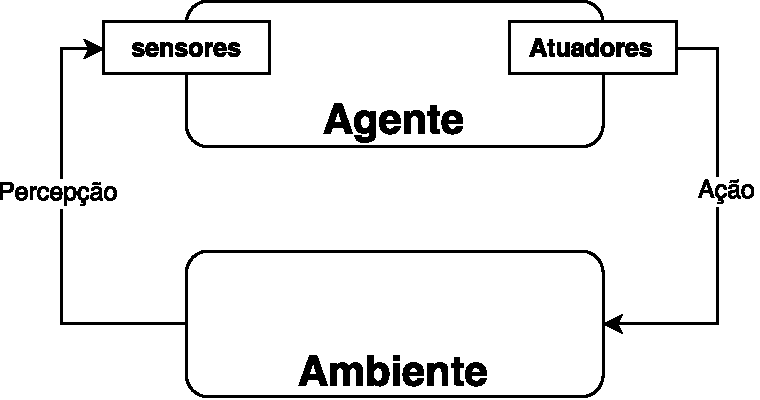
\includegraphics[width=0.6\textwidth]{fig/agente.pdf}
	\caption{Representação de um agente}
	\label{fig:agente}
\end{figure} 

Definindo os agentes como autônomos, eles devem ser capazes de aprender a lidar com as situações proporcionadas pelo ambiente, e serem ativos. \frm{I cannot parse this sentence...}
Para que o agente consiga cumprir estes aspectos é preciso que ele seja capaz de realizar uma ação de forma autônoma e flexível, para que isso aconteça, um agente precisa de três atributos\cite{agent1999}\frm{Como se \emph{cumpre} um aspecto?!?!}: 

\begin{itemize}
	\item reatividade, para que os agentes sejam capazes de perceber o ambiente e suas mudanças a fim de levar o ambiente em consideração para a tomada de decisão das ações;
	\item pró-atividade, para que os agentes consigam ter a iniciativa em tomar as suas ações; e
	\item habilidade social, para que os agentes sejam capazes de interagir com outros agentes(humanos ou não).
\end{itemize}

Os dois primeiros atributos são necessários para que o agente consiga interagir com o ambiente. 
Já o terceiro atributo é necessário para que o agente consiga interagir com outros agentes, pois ele nem sempre vai estar sozinho no ambiente, quando há mais de um agente no sistema, podemos considerar o sistema como multi agentes, onde os agentes interagem entre si. \frm{ Separar as idéias!!}
Os agentes podem ter objetivos em comum ou não, mas o mais importante é que eles terão que, dependendo da situação, cooperar ou negociar entre si \cite{intelligence2003modern}.\frm{Tentando comprimir idéias demais em uma frase só!!}

\section{Arquiteturas de Agentes}
A definição \frm{Que definição? Eu não vi nada falando de definição...} acima é uma forma geral de descrever um agente: um agente recebe um estimulo do ambiente com seus sensores e retorna uma ação por meio de seus atuadores. 
Existem diferentes tipos de arquiteturas de agentes que acrescentam detalhes à forma geral de definir agentes. 
Cada tipo de arquitetura combina componentes diferentes para gerar as ações \cite{intelligence2003modern}. Os quatro tipos básicos de arquiteturas de agentes, que englobam as principais características de agentes são \cite{intelligence2003modern}: 

\begin{itemize}
	\item agentes simples de reflexo (\emph{simple reflex agents});
	\item agentes de reflexo baseados em modelo (\emph{model-based reflex agents});
	\item agentes baseados em objetivo (\emph{goal-based agents}); e
	\item agentes baseados em utilidade (\emph{utility-based agents}). \frm{Termos em língua estrangeira, sempre em itálico.}
\end{itemize}  

\subsection{Simple reflex agents}
\todo[inline,color=red!80]{Tu só reorganizou as frases do livro (e traduziste alguns conceitos meio torto ``occur even in more complex environments'' $\rightarrow$ ``ambientes de alta complexidade'')!! Isto tem que ter vindo do teu entendimento!! Parei de ler no meio quando notei as similaridades com o Russel e Norvig. Repense estas seções, talvez valha a pena comprimir isto.}
A arquitetura considerada a mais simples é a de agentes simples de reflexo. 
Esses agentes escolhem suas ações baseados na percepção atual vinda do ambiente, ignorando qualquer outra percepção que já tenha sido observada~\cite{intelligence2003modern}. 
A Figura~\ref{fig:agenteSimple}\frm{Coloque as figuras em uma escala adequada.} ilustra esse tipo de arquitetura. \frm{Mexi de novo na (figura $\rightarrow$ Figura) e no \emph{ilustra}, não vou mexer mais e deixo isto contigo.}

\begin{figure}[ht]
	\centering
	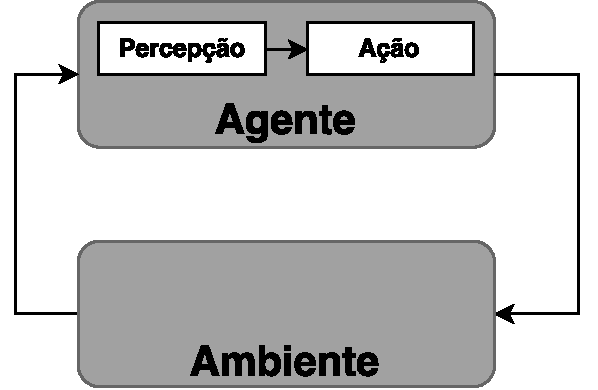
\includegraphics[width=0.4\textwidth]{fig/agentSimple.pdf}
	\caption{Simple reflex agents}
	\label{fig:agenteSimple}
\end{figure} 

\frm{Essa, esse, esse, essa}
Essa arquitetura pode ser usada em ambientes de alta complexidade\frm{?!?!?!?}, como por exemplo, em carros que são dirigidos por agentes, quando o carro da frente freia, o agente deve frear também para não ocasionar em uma batida. \frm{Sério? Por que isto me parece uma afirmação contra a intuição. Tu tens que explicar isto.} 
Esse agente utiliza uma regra de ação condicional, se acontecer uma freada no carro da frente então eu devo frear também. 
Este tipo de agente tem a propriedade de ser simples, mas com isso sua inteligencia fica limitada \cite{intelligence2003modern}\frm{Citando muito livros!! Tentar usar a fonte original, e quando citar livro, incluir o capítulo.}. Essa abordagem é eficaz somente se o ambiente for completamente observável, ou seja, os sensores do agente tem acesso a todas as informações do ambiente a qualquer instante de tempo para detectar aspectos que são relevantes para a escolha das ações, por exemplo, um agente precisa se locomover de uma cidade para a outra, se o ambiente é completamente observável o agente consegue ver todas as estradas que chegam a cidade destino, já se o ambiente for parcialmente observável, pode ter alguma estrada que o agente não consiga ver, e se o agente não consegue ver nenhuma estrada o ambiente é não observável \cite{intelligence2003modern}. \frm{Mega frase com diversas linhas de pensamento. Separar as idéias}

\subsection{Model-based reflex agents}

Os agentes de reflexos baseados em modelo utilizam um estado interno para marcar qual o estado do ambiente ele está. Este estado é utilizado como parte do processo de escolha da ação. A informação do estado pode ser de alguma informação que não pode ser obtida por alguma percepção do ambiente ou de estados que já foram visitados pelo agente. Este tipo de abordagem é eficaz para ambientes parcialmente observáveis, pelo fato de que o estado pode guardar informações relevantes para o agente \cite{intelligence2003modern}. Um modelo deste tipo de agente pode ser visto na figura \ref{fig:agenteModelbased}. 

\begin{figure}[ht]
	\centering
	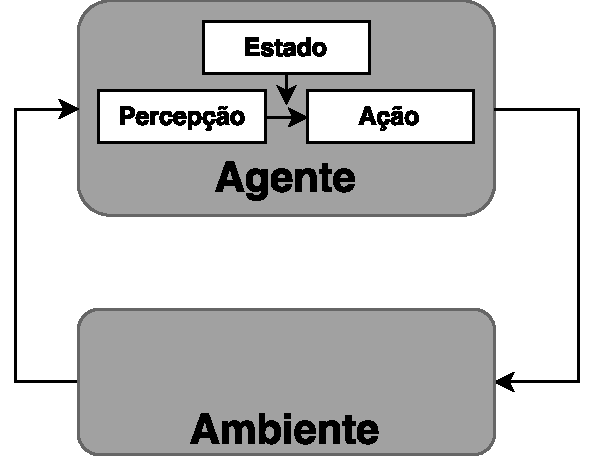
\includegraphics[width=0.6\textwidth]{fig/agentModel.pdf}
	\caption{Model-based reflex agents}
	\label{fig:agenteModelbased}
\end{figure} 

\subsection{Goal-based agents}

Conhecendo o estado atual do ambiente, as vezes, não é suficiente para saber o que fazer \cite{intelligence2003modern}. Além do estado atual, o agente pode precisar de uma informação para saber a onde ele quer chegar, ou seja, um objetivo para descrever o que o agente está buscando alcançar. O objetivo pode ser alcançado com uma ação, outras vezes é mais complicado e leva várias ações. Esta arquitetura é diferente das outras duas apresentadas, pelo fato de se preocupar com o futuro. Para achar a sequencia de ações que alcança o objetivo pode ser usado Busca ou Planejamento, que são sub áreas da IA que tem como objetivo achar a sequencia de ações que levem o agente para o objetivo \cite{intelligence2003modern}. A figura \ref{fig:agenteGoal} mostra a arquitetura e como o objetivo influencia na escolha da ação. 

\begin{figure}[ht]
	\centering
	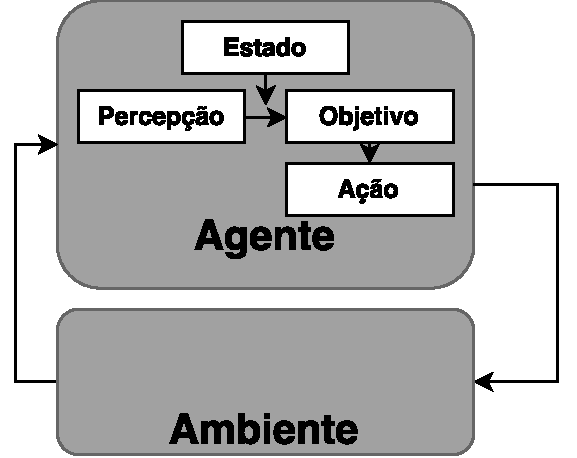
\includegraphics[width=0.6\textwidth]{fig/agenteGoal.pdf}
	\caption{Goal-based agents}
	\label{fig:agenteGoal}
\end{figure} 

\subsection{Utility-based agents}

Apenas alcançar um objetivo pode não ser suficiente para alguns cenários, como por exemplo, um agente que deseja chegar a determinada cidade, existem mais de um caminho que levam para a mesma cidade, indo pelo caminho mais longo o agente ainda estará chegando no objetivo. Para o agente conseguir alcançar o objetivo com uma melhor performance é utilizado uma função de utilidade, nela é medido o "desejo" do agente em tomar determinada ação. Cada ação exercida pelo agente terá influencia no valor de utilidade obtido \cite{intelligence2003modern}. Esta arquitetura é melhor utilizada em ambientes parcialmente observáveis e estocásticos, um ambiente estocástico é onde não há conhecimento preciso do próximo estado dado determinada ação \cite{intelligence2003modern}. A figura \ref{fig:agenteUtility} representa essa arquitetura.  

\begin{figure}[ht]
	\centering
	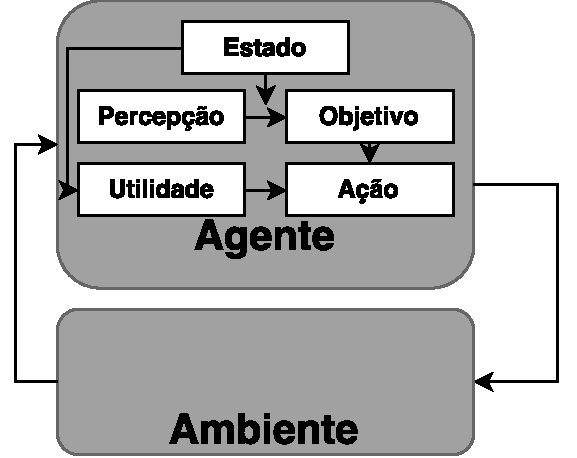
\includegraphics[width=0.6\textwidth]{fig/agentUtility.pdf}
	\caption{Utility-based agents}
	\label{fig:agenteUtility}
\end{figure} 


